\section{The Unified VED$\times$IFGT Equation}
\label{sec:unified_equation}

The evolution equation~\eqref{eq:basic} of the information field introduced in the previous section does not specify the concrete construction of $\sigma$. In this section, we expand $\sigma$ as the mismatch between the difference chain and the existing trace structure, and ultimately unify the formulation into a single equation for VED's closure-degree field $C(x,\tau)$.

\subsection{Expansion of the generation term \texorpdfstring{$\sigma$}{sigma}}
\label{subsec:sigma_expansion}

$\sigma$ consists of three contributions.

\paragraph{(i) Driving term --- supply of unclosed difference.}
In regions where differences have not yet been incorporated into closure, new quasi-closures are generated. This contribution is proportional to the closure margin $(1 - C/C_*)$ and the difference source $\Delta$:
\begin{equation}
\sigma_{\mathrm{drive}} = a \, \Delta \, \left(1 - C/C_*\right).
\label{eq:sigma_drive}
\end{equation}
Here $\Delta$ denotes the difference source in VED (see~§\ref{subsec:difference}), $a$ is the generation rate, and $C_*$ is the effective closure upper bound. As $C \to C_*$, the driving vanishes.

\paragraph{(ii) Dissipation term --- collapse of traces.}
Quasi-closures decay over time, either being reabsorbed into closure or being released again as difference. This contribution is proportional to the trace density (equivalently, the local strength of $C$):
\begin{equation}
\sigma_{\mathrm{dissip}} = -\Gamma \, C,
\label{eq:sigma_dissip}
\end{equation}
where $\Gamma$ is the dissipation rate.

\paragraph{(iii) Barrier term --- the prohibition of complete closure.}
As a basic principle of VED, complete closure at $C = C_{\max} = 1$ is prohibited. This is a structural constraint that follows from the foundational axiom ``\emph{there is difference}.'' The prohibition is expressed as a repulsive potential that diverges as $C \to C_{\max}$:
\begin{equation}
\sigma_{\mathrm{barrier}} = -\frac{\kappa_B}{C_{\max} - C},
\label{eq:sigma_barrier}
\end{equation}
where $\kappa_B$ is the barrier strength. This term prevents asymptotic approach to complete closure and ensures circulation as a quasi-closure.

The three contributions are visualized in Fig.~\ref{fig:sigma_decomposition}.

\begin{figure}[h]
  \centering
  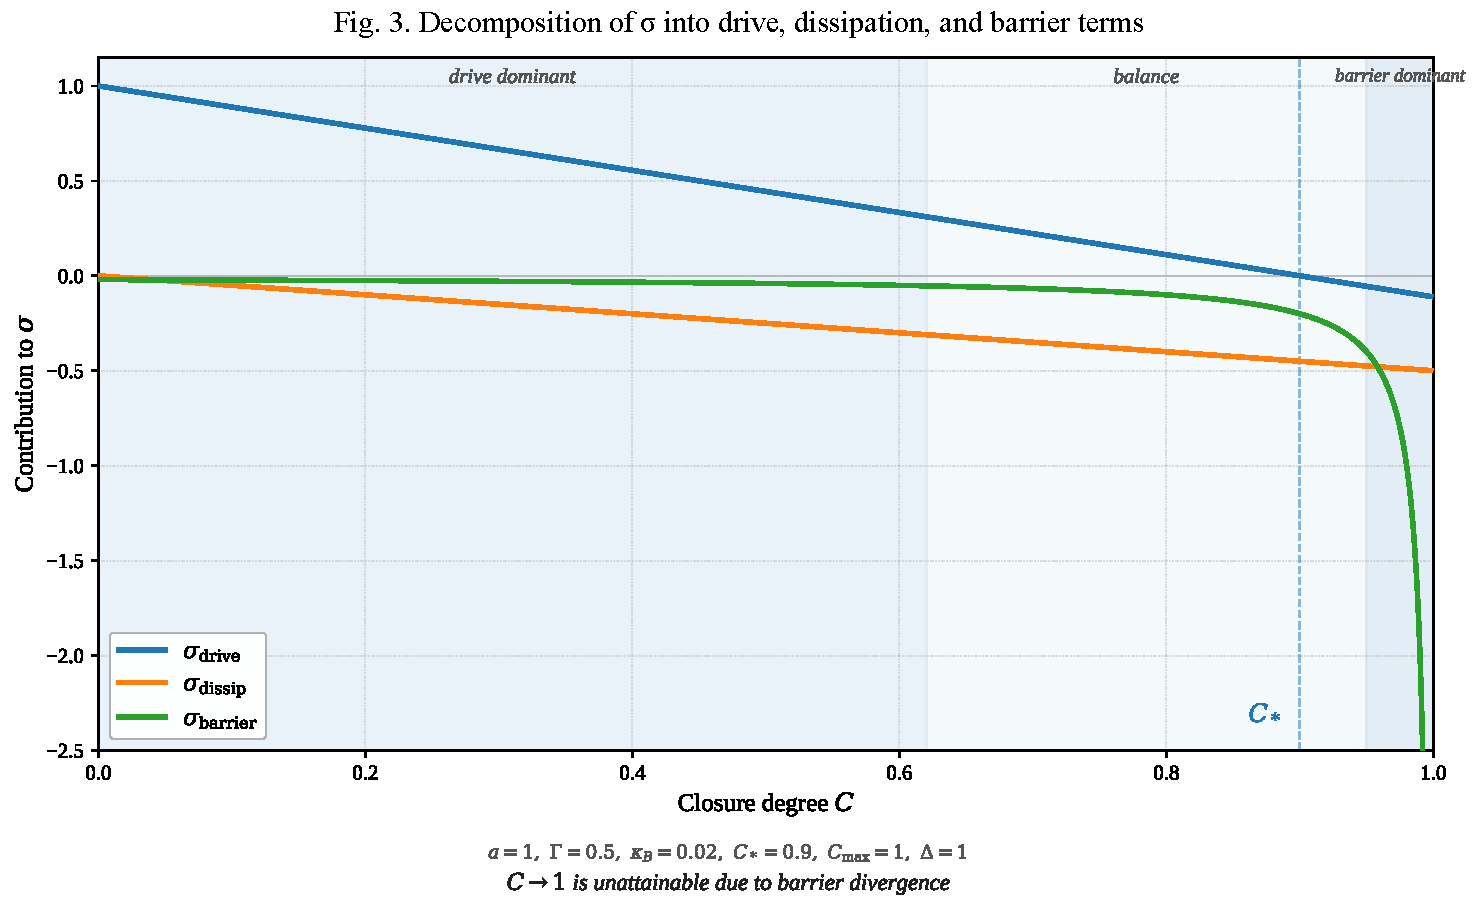
\includegraphics[width=0.95\textwidth]{figures/fig3_sigma_decomposition_en.pdf}
  \caption{Decomposition of $\sigma$ into drive, dissipation, and barrier terms. The barrier term diverges as $C \to 1$, ensuring that complete closure is unattainable.}
  \label{fig:sigma_decomposition}
\end{figure}

\subsection{The unified VED$\times$IFGT equation}
\label{subsec:unified_eq}

Substituting the above into~\eqref{eq:basic} and expressing the information density $I$ as a function of $C$, we obtain a single evolution equation for the closure-degree field $C(x,\tau)$.

For the relation between $I$ and $C$, we adopt the \emph{linear assumption} as the leading-order approximation:
\begin{equation}
I = f(1 - C) = 1 - C.
\label{eq:linear_assumption}
\end{equation}
Nonlinear corrections $f(x) = x + O(x^2)$ are left for future work. Under this assumption, $\nabla I = -\nabla C$, and the sign is inverted when the information flow $J$ is rewritten as the closure flow $J_C$.

Substituting into~\eqref{eq:basic}, we obtain the following unified equation:
\begin{equation}
\boxed{
\frac{\partial C}{\partial \tau} + \nabla \cdot J_C
= a \, \Delta \, \left(1 - C/C_*\right) - \Gamma \, C - \frac{\kappa_B}{C_{\max} - C}
}
\label{eq:unified}
\end{equation}
\begin{equation}
J_C = -D \nabla C - \mu \alpha \, C \nabla C.
\label{eq:J_C}
\end{equation}
The second term on the right-hand side of~\eqref{eq:J_C} originates from the constraint potential gradient $F_I = \alpha \nabla C$ given in~\eqref{eq:F_I}, rewritten in terms of $C$ under the linear assumption~\eqref{eq:linear_assumption}.

\paragraph{On the temporal argument.}
The time derivative in~\eqref{eq:unified} is taken with respect to the informational time $\tau$ (see~§\ref{subsec:time}), which is not an external parameter defined on a background spacetime. $\tau$ is generated endogenously from the update process of the closure-degree field $C$ itself; in this sense,~\eqref{eq:unified} is an equation that internalizes the generative process of time.

However, in the approximate regime in which $C$ is sufficiently mature and the background spacetime may be regarded as nearly fixed, $\tau$ can be replaced by an external time $t$:
\begin{equation}
\frac{\partial C}{\partial t} + \nabla \cdot J_C = \cdots,
\label{eq:unified_external}
\end{equation}
and this form is directly comparable with existing reaction--diffusion equations and Ginzburg--Landau-type equations. In this paper, the $\tau$-form~\eqref{eq:unified} is taken as fundamental, while the $t$-form~\eqref{eq:unified_external} is positioned as an effective description.

\subsection{Interpretation of the unified equation}
\label{subsec:interpretation}

Equation~\eqref{eq:unified} could, in principle, generate an extremely broad class of structures from the single field $C(x,\tau)$. Although detailed analysis is beyond the scope of this paper, we list below, as a guide for future development, the directions in which structures might be identified. Note that when ``circulation'' or ``limit cycle'' is mentioned below, it refers to circulation as a solution of equation~\eqref{eq:unified}; this is a different level of discourse from the conceptual circulation between VED and IFGT described in~§\ref{subsec:circular}.

\begin{itemize}
  \item \textbf{Spatial structure} --- potentially corresponding to smooth gradient regions of $\nabla C$.
  \item \textbf{Temporal structure} --- potentially corresponding to the $\tau$-evolution as a relaxation process.
  \item \textbf{Particle-like structure} --- potentially corresponding to deeply localized stable solutions (regions where $C$ is locally close to $C_*$).
  \item \textbf{Meaning-like structure} --- potentially corresponding to shallowly localized metastable solutions (regions where $C$ stays at intermediate values).
  \item \textbf{Life-like structure} --- potentially corresponding to limit-cycle-type circulatory solutions.
  \item \textbf{Intelligence-like structure} --- potentially corresponding to nontrivial global solutions involving closure reconfiguration.
\end{itemize}

These may all be positioned as distinct solution classes of~\eqref{eq:unified}, but their individual identification and derivation lie beyond the scope of this paper. Under the division of roles in which VED handles generation, IFGT handles structure, and the unified equation~\eqref{eq:unified} bridges the two through dynamics, these concrete correspondences will be developed in separate works.

\subsection{The minimal axiom system}
\label{subsec:minimal_axioms}

Equation~\eqref{eq:unified} is derived from the following \emph{two axioms}:

\begin{enumerate}
  \item \emph{There is difference.} (the foundational axiom of VED)
  \item \emph{Difference tends to close.} (the additional axiom of IFGT)
\end{enumerate}

From the first axiom, the driving and barrier terms are derived; from the second, the dissipation term and the construction of the information flow are derived. The unified VED$\times$IFGT system is thus built upon these two minimal axioms.
